\documentclass{beamer}
%------------------------------------------------------------
% Theme and Appearance
%------------------------------------------------------------
\usetheme[]{Boadilla} 
\usecolortheme{default}
\setbeamertemplate{navigation symbols}{} 
% Headline with Access Code
\setbeamertemplate{headline}{
    \begin{beamercolorbox}[wd=\paperwidth,ht=2.5ex,dp=1ex,right]{section in head/foot}
        \usebeamerfont{section in head/foot}
        \hspace{0.5cm}
        \ifnum\insertframenumber<20
            \raisebox{-1pt}[0pt][0pt]{\normalsize\textbf{Access Code: 123456}}
        \fi
        \hspace{0.5cm}
    \end{beamercolorbox}
}
\usepackage[utf8]{inputenc}
\usepackage{minted}
\usepackage{lmodern}
\usepackage{tgheros}
\usepackage{hyperref}
\usepackage{tikz}
\usetikzlibrary{shapes, arrows, positioning, shadows}

\renewcommand*\familydefault{\sfdefault}

% Agenda at the start of every section
\AtBeginSection[]
{
    \begin{frame}
        \frametitle{Agenda}
        \tableofcontents[currentsection]
    \end{frame}
}

%------------------------------------------------------------
% Title Page Information
%------------------------------------------------------------
\title[CMP9134 - Week 1]{Version Control Systems: Git \& GitHub}
\subtitle{CMP9134: Software Engineering}
\author[fdelduchetto]{Dr Francesco Del Duchetto\\Lecturer in Robotics and Autonomous Systems}
\institute[UoL]{University of Lincoln}
\date{6 February 2026}

%------------------------------------------------------------
\begin{document}

%--- TITLE FRAME ---
\begin{frame}
    \titlepage
\end{frame}

%--- AGENDA FRAME ---
\begin{frame}
    \frametitle{Lab Session's Agenda}
    \tableofcontents
\end{frame}

%--- LEARNING AIMS ---
% \begin{frame}
%     \frametitle{Learning Aims}
%     By the end of this session, you will be able to:
%     \begin{itemize}
%         \item Explain \textbf{why} we use Version Control.
%         \item Understand the \textbf{Three States of Git} (Working, Staging, Repo).
%         \item Perform the core cycle: \textbf{Add} $\rightarrow$ \textbf{Commit} $\rightarrow$ \textbf{Push}.
%         \item Create and connect a \textbf{Remote Repository} on GitHub.
%     \end{itemize}
% \end{frame}

%=============================================================
\section{Why Version Control?}
%=============================================================

\begin{frame}
    \frametitle{The "Copy-Paste" Method}
    \begin{columns}
        \column{0.5\textwidth}
        \begin{center}
            \textit{"I'll just make a copy of the folder before I try this risky change..."}
        \end{center}
        \textbf{The Result:}
        \begin{itemize}
            \item Hard to find the right file.
            \item Wastes disk space.
            \item "Which 'Final' is the real one?"
        \end{itemize}
        
        \column{0.5\textwidth}
        \begin{center}
        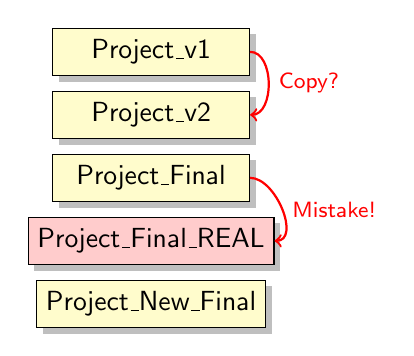
\begin{tikzpicture}[
            file/.style={draw, fill=yellow!20, rectangle, minimum width=2.5cm, minimum height=0.6cm, drop shadow},
            node distance=0.8cm
        ]
            \node[file] (f1) {Project\_v1};
            \node[file, below of=f1] (f2) {Project\_v2};
            \node[file, below of=f2] (f3) {Project\_Final};
            \node[file, below of=f3, fill=red!20] (f4) {Project\_Final\_REAL};
            \node[file, below of=f4] (f5) {Project\_New\_Final};
            
            \draw[->, thick, red] (f1.east) to[out=0,in=0] node[midway, right, font=\footnotesize] {Copy?} (f2.east);
            \draw[->, thick, red] (f3.east) to[out=0,in=0] node[midway, right, font=\footnotesize] {Mistake!} (f4.east);
        \end{tikzpicture}
        \end{center}
    \end{columns}
\end{frame}

\begin{frame}
    \frametitle{Collaboration}
    \textbf{The Scenario:} You and a teammate are working on the same codebase.
    \begin{itemize}
        \item You both make changes to the same file.
        \item You email each other the updated files.
        \item You accidentally overwrite each other's work.
        \item Now you have two conflicting versions of the same file.
        \item Who has the latest changes? How do you merge? How do you keep track of who did what? ...
    \end{itemize}
\end{frame}

\begin{frame}
    \frametitle{The Solution: Version Control Systems (VCS)}
    
    A VCS is a system that records changes to a file system over time.
    
    \vspace{0.3cm}
    \textbf{Key Benefits:}
    \begin{enumerate}
        \item \textbf{History:} You can see exactly \textit{who} changed \textit{what} and \textit{when}.
        \item \textbf{Revert:} Made a mistake? Go back to yesterday's version instantly.
        \item \textbf{Collaboration:} Multiple people can work on the same file without overwriting each other.
        \item \textbf{Backup:} Your code exists on your machine AND the cloud.
    \end{enumerate}
\end{frame}

%=============================================================
\section{Version Control Systems}
%=============================================================

\begin{frame}
    \frametitle{What is a Version Control System (VSC)?}
    Is a program/set of tools that help you manage changes to files over time.
    \begin{center}
    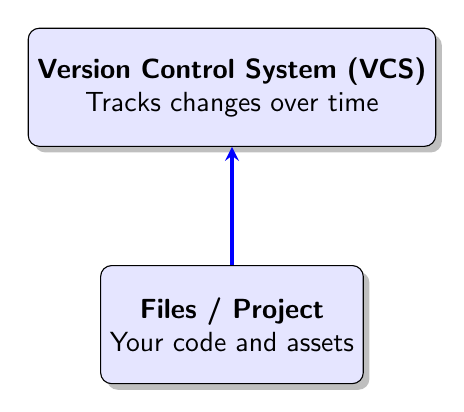
\begin{tikzpicture}[
        box/.style={draw, rectangle, rounded corners, minimum width=3cm, minimum height=1.5cm, align=center, fill=blue!10, drop shadow},
        arrow/.style={->, >=stealth, very thick}
    ]
        \node[box] (vcs) {\textbf{Version Control System (VCS)}\\Tracks changes over time};
        \node[box, below=1.5cm of vcs] (files) {\textbf{Files / Project}\\Your code and assets};  
        \draw[arrow, blue] (files.north) -- (vcs.south);
    \end{tikzpicture}
    \end{center}
\end{frame}

\begin{frame}
    \frametitle{What is a Version Control System (VSC)?}
    VSC systems allow several team members to work on the same project simultaneously.
    \begin{center}
    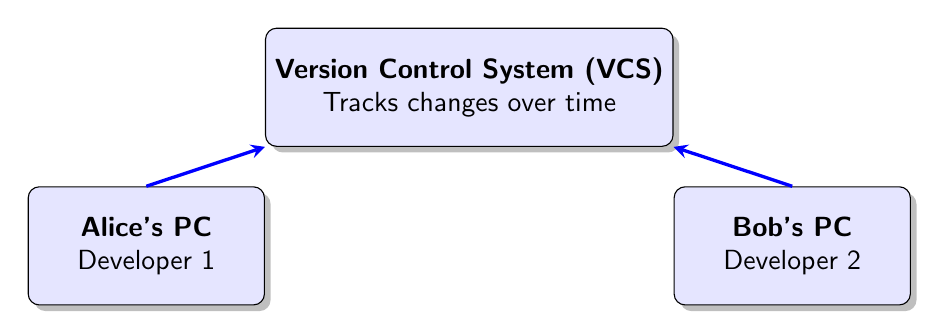
\begin{tikzpicture}[
        box/.style={draw, rectangle, rounded corners, minimum width=3cm, minimum height=1.5cm, align=center, fill=blue!10, drop shadow},
        arrow/.style={->, >=stealth, very thick}
    ]
        \node[box] (vcs) {\textbf{Version Control System (VCS)}\\Tracks changes over time};
        \node[box, below left=0.5cm and 0cm of vcs] (alice) {\textbf{Alice's PC}\\Developer 1};
        \node[box, below right=0.5cm and 0cm of vcs] (bob) {\textbf{Bob's PC}\\Developer 2};  
        \draw[arrow, blue] (alice.north) -- (vcs.south west);
        \draw[arrow, blue] (bob.north) -- (vcs.south east);
    \end{tikzpicture}
    \end{center}
    \vspace{0.3cm}
    Each developer has a local copy of the project and can make changes independently.
\end{frame}


\begin{frame}
    \frametitle{Popular Version Control Systems}
    \begin{itemize}
        \item \textbf{Git:} The most widely used VCS today. Created by Linus Torvalds (creator of linux) in 2005 for Linux kernel development.
        \item \textbf{Subversion (SVN):} An older centralized VCS, still used in some legacy projects.
        \item \textbf{Mercurial:} Similar to Git, but with a different design philosophy.
        \item \textbf{Perforce:} A commercial VCS often used in large enterprises and game development.
    \end{itemize}
    \vspace{0.3cm}
    In this lecture, we will focus on \textbf{Git} and its cloud counterpart, \textbf{GitHub}.

    \vspace{0.3cm}
    If you are curious about what ``git'' stands for, have a look at the first definition from the creator: \url{https://github.com/git/git/blob/e83c5163316f89bfbde7d9ab23ca2e25604af290/README}
\end{frame}


\begin{frame}
    \frametitle{Centralized vs Distributed VCS}
    \textbf{Centralized VCS:}
    \begin{itemize}
        \item A single central server stores all versions of the project.
        \item Developers check out files from this central place.
        \item Examples: Subversion (SVN), Perforce.
    \end{itemize}
    
    \vspace{0.3cm}
    \textbf{Distributed VCS:}
    \begin{itemize}
        \item Every developer has a full copy of the entire repository (including history).
        \item Changes can be shared between repositories.
        \item Examples: Git, Mercurial.
    \end{itemize}
    
    \vspace{0.3cm}
    Most modern VCS (including Git) are distributed, offering greater flexibility and offline capabilities.
\end{frame}


\begin{frame}
    \frametitle{Git vs GitHub: The Distinction}
    
    \begin{columns}
        \column{0.5\textwidth}
        \textbf{Git (The Engine)}
        \begin{itemize}
            \item A command-line tool installed on your laptop.
            \item Tracks history locally.
            \item Does not need internet.
            \item \textit{Analogy: Microsoft Word}
        \end{itemize}
        
        \column{0.5\textwidth}
        \textbf{GitHub (The Host)}
        \begin{itemize}
            \item A website (cloud service).
            \item Hosts Git repositories online.
            \item Adds social features (Teams, Pull Requests).
            \item \textit{Analogy: Google Drive / Dropbox}
        \end{itemize}
    \end{columns}
\end{frame}

\begin{frame}
    \frametitle{The Three States of Git}
    Files move through three "zones".
    
    \vspace{0.5cm}
    \begin{center}
    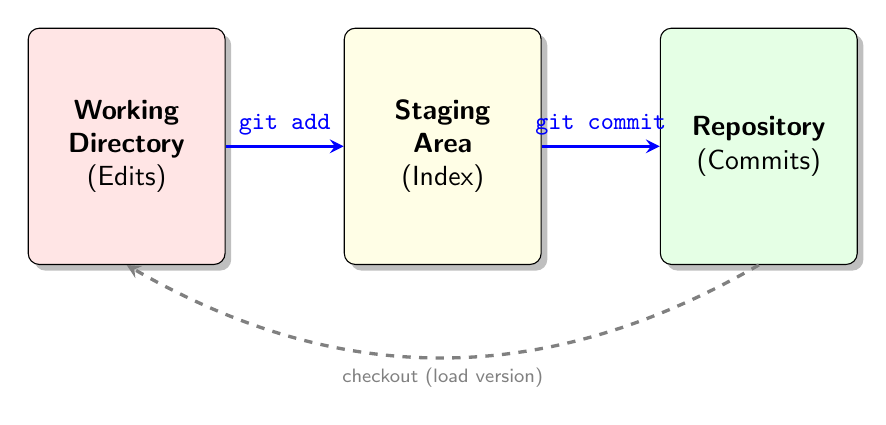
\begin{tikzpicture}[
        zone/.style={draw, rectangle, rounded corners, minimum width=2.5cm, minimum height=3cm, align=center, drop shadow},
        arrow/.style={->, >=stealth, very thick}
    ]
        % Zones
        \node[zone, fill=red!10] (working) {\textbf{Working}\\\textbf{Directory}\\(Edits)};
        \node[zone, fill=yellow!10, right=1.5cm of working] (staging) {\textbf{Staging}\\\textbf{Area}\\(Index)};
        \node[zone, fill=green!10, right=1.5cm of staging] (repo) {\textbf{Repository}\\(Commits)};

        % Arrows
        \draw[arrow, blue] (working) -- node[above, font=\small\ttfamily] {git add} (staging);
        % Diagram documentation:
        % - Visualizes a simple Git workflow with three areas: Working, Staging, Repository.
        % - Nodes:
        %   * Working: your editable files (working directory).
        %   * Staging: the index where you prepare changes to be committed.
        %   * Repository: the permanent commit history (local .git).
        %
        % - Arrows:
        %   * Solid blue arrow labeled "git commit" (staging -> repository):
        %     Represents creating a new commit from the staged changes, recording a snapshot in the repository.
        %   * Dashed gray arrow labeled "checkout (load version)" (repository -> working):
        %     Represents loading a version from the repository into the working directory.
        %
        % Explanation of the "checkout" arrow:
        % - "Checkout" means updating the working tree to match a specific commit/branch or file version stored in the repository.
        % - It reads data from the repository and writes files into the Working area, and typically updates HEAD to point to the selected branch/commit.
        % - It does not create new commits in the repository; it changes which commit is checked out and what files you see/edit locally.
        % - The dashed style indicates a read/load operation (bringing a stored version into the working copy) rather than creating or saving history.
        \draw[arrow, blue] (staging) -- node[above, font=\small\ttfamily] {git commit} (repo);
        
        % Check out arrow
        \draw[arrow, dashed, gray] (repo.south) to[bend left] node[below, font=\scriptsize] {checkout (load version)} (working.south);
        %out=240,in=300]
    \end{tikzpicture}
    \end{center}
    
    \begin{itemize}
        \item \textbf{1. Working:} Where you create and edit files.
        \item \textbf{2. Staging:} Where you select files to be saved.
        \item \textbf{3. Repository:} Where the permanent snapshot is stored.
    \end{itemize}
\end{frame}

%=============================================================
% \section{Essential Terminal Commands}
%=============================================================
%=============================================================
\section{The Core Cycle: Status, Add, Commit}
%=============================================================

\begin{frame}[fragile]
    \frametitle{The Terminal: Your New Best Friend}
    Git is primarily a \textbf{Command Line Interface (CLI)} tool.
    
    \vspace{0.3cm}
    \begin{columns}
        \column{0.6\textwidth}
            \textbf{1. Where am I?}
            \begin{minted}[fontsize=\footnotesize]{bash}
pwd  # Print Working Directory
ls   # List Files
            \end{minted}
            
            \vspace{0.2cm}
            \textbf{2. Moving Around}
            \begin{minted}[fontsize=\footnotesize]{bash}
cd FolderName  # Enter folder
cd ..          # Go back/up
            \end{minted}
            
            \vspace{0.2cm}
            \textbf{3. Creating}
            \begin{minted}[fontsize=\footnotesize]{bash}
mkdir NewProject # Make folder
touch file.txt   # Create file
            \end{minted}
            
        \column{0.4\textwidth}
            \begin{center}
            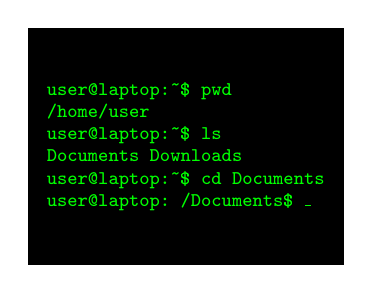
\begin{tikzpicture}
                \node[draw, fill=black, text=green, font=\ttfamily\scriptsize, align=left, minimum width=4cm, minimum height=3cm] {
                    user@laptop:\textasciitilde\$ pwd\\
                    /home/user\\
                    user@laptop:\textasciitilde\$ ls\\
                    Documents Downloads\\
                    user@laptop:\textasciitilde\$ cd Documents\\
                    user@laptop:~/Documents\$ \_
                };
            \end{tikzpicture}
            \end{center}
    \end{columns}
\end{frame}


\begin{frame}[fragile]
    \frametitle{Step 1: Check Status}
    
    \textbf{Rule \#1 of Git:} If you are confused, type \texttt{git status}.
    
    \begin{minted}[fontsize=\small]{bash}
git status
    \end{minted}
    
    \vspace{0.3cm}
    It tells you:
    \begin{itemize}
        \item \textcolor{red}{Red Files}: Modified but not staged (Working Directory).
        \item \textcolor{green}{Green Files}: Staged and ready to commit (Staging Area).
        \item "Nothing to commit": Everything is saved.
    \end{itemize}
\end{frame}

\begin{frame}[fragile]
    \frametitle{Step 2: Staging Files (Add)}
    
    We move files from "Working" to "Staging".
    
    \begin{minted}[fontsize=\small]{bash}
# Add a single file
git add Program.cs

# Add EVERYTHING (The most common command)
git add .
    \end{minted}
    
    \vspace{0.3cm}
    \textbf{Why separate steps?}
    Sometimes you modify 10 files, but you only want to save 5 of them as a specific update (e.g., "Fix login bug"). You stage only the login files.
\end{frame}

\begin{frame}[fragile]
    \frametitle{Step 3: Committing (Save)}
    
    We seal the Staged files into a permanent snapshot.
    
    \begin{minted}[fontsize=\small]{bash}
git commit -m "Added the main menu logic"
    \end{minted}
    
    \vspace{0.3cm}
    \textbf{The Commit Message (\texttt{-m}):}
    \begin{itemize}
        \item Mandatory.
        \item Be descriptive! "Fixed bug" is bad. "Fixed divide-by-zero error" is good.
    \end{itemize}

    \vspace{0.3cm}
    You can check the history of commits in your repository with:
    \begin{minted}[fontsize=\small]{bash}
git log
    \end{minted}

\end{frame}

\begin{frame}
    \frametitle{The Core Cycle Recap}
    
    \begin{center}
    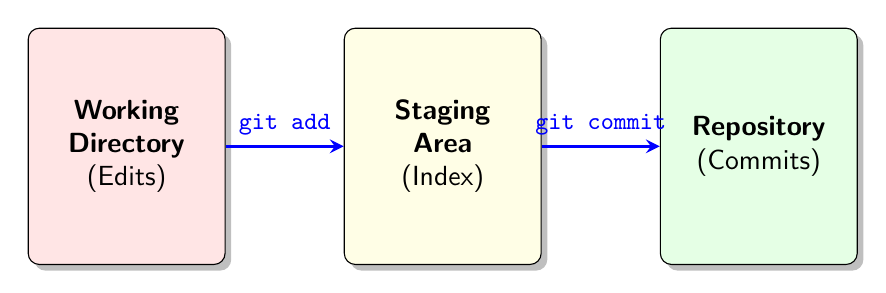
\begin{tikzpicture}[
        zone/.style={draw, rectangle, rounded corners, minimum width=2.5cm, minimum height=3cm, align=center, drop shadow},
        arrow/.style={->, >=stealth, very thick}
    ]
        % Zones
        \node[zone, fill=red!10] (working) {\textbf{Working}\\\textbf{Directory}\\(Edits)};
        \node[zone, fill=yellow!10, right=1.5cm of working] (staging) {\textbf{Staging}\\\textbf{Area}\\(Index)};
        \node[zone, fill=green!10, right=1.5cm of staging] (repo) {\textbf{Repository}\\(Commits)};

        % Arrows
        \draw[arrow, blue] (working) -- node[above, font=\small\ttfamily] {git add} (staging);
        \draw[arrow, blue] (staging) -- node[above, font=\small\ttfamily] {git commit} (repo);
        
    \end{tikzpicture}
    \end{center}
    
    \begin{itemize}
        \item \textbf{1. Status:} Check what's happening (\texttt{git status}).
        \item \textbf{2. Add:} Stage files (\texttt{git add .}).
        \item \textbf{3. Commit:} Save snapshot (\texttt{git commit -m "..."}).
    \end{itemize}
\end{frame}


\section{Reverting to Previous Versions}

\begin{frame}[fragile]
    \frametitle{Understanding Commits}
    
    Each commit has a unique ID (hash).
    
    \vspace{0.3cm}
    \textbf{View Commit History:}
    \begin{minted}[fontsize=\small]{bash}
git log
    \end{minted}
    \vspace{0.3cm}
    \textbf{Sample Output:}
    \begin{minted}[fontsize=\small]{text}
commit a1b2c3d4e5f6g7h8i90jklmnopqrstuv
Author: Your Name <email>
Date:   Mon Jan 12 10:00:00 2026 +0000

    Added the main menu logic
    \end{minted}

    \vspace{0.3cm}

    \begin{center}
    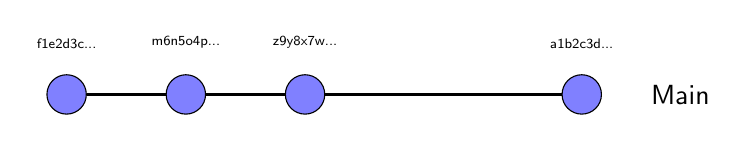
\begin{tikzpicture}[
        commit/.style={circle, draw, fill=blue!50, minimum size=0.5cm, inner sep=0pt},
        feature/.style={circle, draw, fill=green!50, minimum size=0.5cm, inner sep=0pt},
        line/.style={-, thick}
    ]
        % Main branch
        \node[commit] (c1) {};
        \node[commit, right=1cm of c1] (c2) {};
        \node[commit, right=1cm of c2] (c3) {};
        \node[commit, right=3cm of c3] (c4) {}; % Gap for feature
        \node[right=0.5cm of c4] (end) {Main};
        
        \node[above=0.2cm of c4, font=\tiny] {a1b2c3d...};
        \node[above=0.2cm of c3, font=\tiny] {z9y8x7w...};
        \node[above=0.2cm of c2, font=\tiny] {m6n5o4p...};
        \node[above=0.2cm of c1, font=\tiny] {f1e2d3c...};
        \draw[line] (c1) -- (c2) -- (c3);
        \draw[line] (c3) -- (c4);
                
        % % Feature branch
        % \node[feature, above right=1cm and 0.5cm of c3] (f1) {};
        % \node[feature, right=1cm of f1] (f2) {};
        % \node[right=0.5cm of f2] (fend) {Feature};

        % \draw[line, green!70!black, ->] (c3) to[out=45, in=180] (f1);
        % \draw[line, green!70!black] (f1) -- (f2);
        % \draw[line, green!70!black, ->] (f2) to[out=0, in=135] (c4);
        
        % \node[above=0.2cm of f1, font=\tiny] {Experiment};
        % \node[below=0.2cm of c4, font=\tiny] {Merge};
        
    \end{tikzpicture}
    \end{center}
\end{frame}

\begin{frame}[fragile]
    \frametitle{Branches}
    \textbf{Branches:} Pointers to specific commits, allowing parallel development.
    \begin{itemize}
        \item \textbf{\texttt{main}}: The default branch.
        \item \texttt{feature-x}: A branch for a new feature.
        \item \texttt{...}
    \end{itemize}

        \textbf{You will see something like:}
    \begin{minted}[fontsize=\small]{text}
commit a1b2c3d4e5f6g7h8i90jklmnopqrstuv (HEAD -> main)
Author: ..
    \end{minted}
    Which means you are currently on the \texttt{main} branch. \texttt{HEAD} points to the latest commit on that branch.
\end{frame} 


\begin{frame}[fragile]
    \frametitle{Reverting to Previous Versions}
    
    If you made a mistake, you can revert to a previous commit.
    
    \vspace{0.3cm}
    \textbf{Find the Commit ID:}
    \begin{minted}[fontsize=\small]{bash}
git log
    \end{minted}
    \vspace{0.3cm}
    \textbf{Revert to that Commit:}
    \begin{minted}[fontsize=\small]{bash}
git checkout z9y8x7w...
    \end{minted}
        \begin{center}
    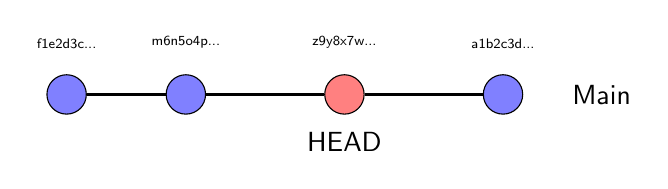
\begin{tikzpicture}[
        commit/.style={circle, draw, fill=blue!50, minimum size=0.5cm, inner sep=0pt},
        head/.style={circle, draw, fill=red!50, minimum size=0.5cm, inner sep=0pt},
        feature/.style={circle, draw, fill=green!50, minimum size=0.5cm, inner sep=0pt},
        line/.style={-, thick}
    ]
        % Main branch
        \node[commit] (c1) {};
        \node[commit, right=1cm of c1] (c2) {};
        \node[head, right=1.5cm of c2] (c3) {};
        \node[commit, right=1.5cm of c3] (c4) {}; % Gap for feature
        \node[right=0.5cm of c4] (end) {Main};
        \node[below=0.1cm of c3] (end) {HEAD};
        
        \node[above=0.2cm of c4, font=\tiny] {a1b2c3d...};
        \node[above=0.2cm of c3, font=\tiny] {z9y8x7w...};
        \node[above=0.2cm of c2, font=\tiny] {m6n5o4p...};
        \node[above=0.2cm of c1, font=\tiny] {f1e2d3c...};
        \draw[line] (c1) -- (c2) -- (c3);
        \draw[line] (c3) -- (c4);        
    \end{tikzpicture}
    \end{center}

\textbf{To return to the latest commit on the main branch:}
    \begin{minted}[fontsize=\small]{bash}
git checkout main
    \end{minted}
            \begin{center}
    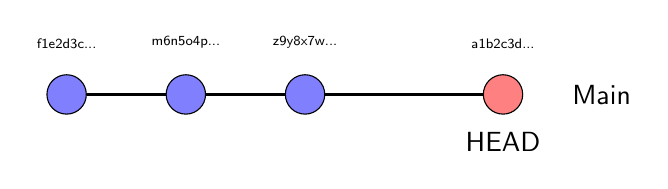
\begin{tikzpicture}[
        commit/.style={circle, draw, fill=blue!50, minimum size=0.5cm, inner sep=0pt},
        head/.style={circle, draw, fill=red!50, minimum size=0.5cm, inner sep=0pt},
        feature/.style={circle, draw, fill=green!50, minimum size=0.5cm, inner sep=0pt},
        line/.style={-, thick}
    ]
        % Main branch
        \node[commit] (c1) {};
        \node[commit, right=1cm of c1] (c2) {};
        \node[commit, right=1cm of c2] (c3) {};
        \node[head, right=2cm of c3] (c4) {}; % Gap for feature
        \node[right=0.5cm of c4] (end) {Main};
        \node[below=0.1cm of c4] (end) {HEAD};
        
        \node[above=0.2cm of c4, font=\tiny] {a1b2c3d...};
        \node[above=0.2cm of c3, font=\tiny] {z9y8x7w...};
        \node[above=0.2cm of c2, font=\tiny] {m6n5o4p...};
        \node[above=0.2cm of c1, font=\tiny] {f1e2d3c...};
        \draw[line] (c1) -- (c2) -- (c3);
        \draw[line] (c3) -- (c4);        
    \end{tikzpicture}
    \end{center}
\end{frame}

\begin{frame}
    \frametitle{Branching: Parallel Universes}
    
    \begin{center}
    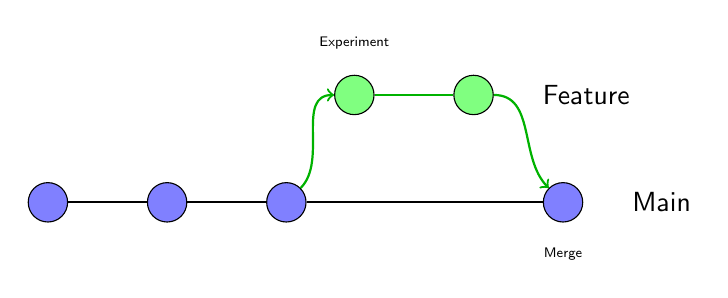
\begin{tikzpicture}[
        commit/.style={circle, draw, fill=blue!50, minimum size=0.5cm, inner sep=0pt},
        feature/.style={circle, draw, fill=green!50, minimum size=0.5cm, inner sep=0pt},
        line/.style={-, thick}
    ]
        % Main branch
        \node[commit] (c1) {};
        \node[commit, right=1cm of c1] (c2) {};
        \node[commit, right=1cm of c2] (c3) {};
        \node[commit, right=3cm of c3] (c4) {}; % Gap for feature
        \node[right=0.5cm of c4] (end) {Main};
        
        \draw[line] (c1) -- (c2) -- (c3);
        \draw[line] (c3) -- (c4);
        
        % Feature branch
        \node[feature, above right=1cm and 0.5cm of c3] (f1) {};
        \node[feature, right=1cm of f1] (f2) {};
        \node[right=0.5cm of f2] (fend) {Feature};

        \draw[line, green!70!black, ->] (c3) to[out=45, in=180] (f1);
        \draw[line, green!70!black] (f1) -- (f2);
        \draw[line, green!70!black, ->] (f2) to[out=0, in=135] (c4);
        
        \node[above=0.2cm of f1, font=\tiny] {Experiment};
        \node[below=0.2cm of c4, font=\tiny] {Merge};
        
    \end{tikzpicture}
    \end{center}
    
    \textbf{The Scenario:} You want to add a feature.
    \begin{itemize}
        \item You work in the \textbf{Feature Branch} (Green).
        \item The \textbf{Main Branch} (Blue) stays safe.
        \item If it works, you \textbf{Merge} it back.
    \end{itemize}
\end{frame}

\begin{frame}[fragile]
    \frametitle{Branching Commands}
    \textbf{Create and switch to a new branch:}
    \begin{minted}[fontsize=\small]{bash}
# Create and Switch to a new branch
git checkout -b feature
# ... write code, add, commit ...
\end{minted}

    \begin{center}
    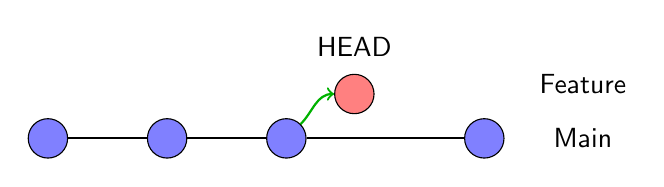
\begin{tikzpicture}[
        commit/.style={circle, draw, fill=blue!50, minimum size=0.5cm, inner sep=0pt},
        feature/.style={circle, draw, fill=red!50, minimum size=0.5cm, inner sep=0pt},
        line/.style={-, thick}
    ]
        % Main branch
        \node[commit] (c1) {};
        \node[commit, right=1cm of c1] (c2) {};
        \node[commit, right=1cm of c2] (c3) {};
        \node[commit, right=2cm of c3] (c4) {}; % Gap for feature
        \node[right=0.5cm of c4] (end) {Main};
        
        \draw[line] (c1) -- (c2) -- (c3);
        \draw[line] (c3) -- (c4);
        
        % Feature branch
        \node[feature, above right=0.2cm and 0.5cm of c3] (f1) {};
        % \node[feature, right=1cm of f1] (f2) {};
        \node[above=0.2cm of end] (fend) {Feature};

        \draw[line, green!70!black, ->] (c3) to[out=45, in=180] (f1);
        % \draw[line, green!70!black] (f1) -- (f2);
        % \draw[line, green!70!black, ->] (f2) to[out=0, in=135] (c4);
        
        \node[above=0.1cm of f1] {HEAD};
        % \node[below=0.2cm of c4, font=\tiny] {Merge};
        
    \end{tikzpicture}
    \end{center}


    \textbf{Switch back to an existing branch:}
    \begin{minted}[fontsize=\small]{bash}
git checkout main
    \end{minted}
    \vspace{0.2cm}

        \begin{center}
    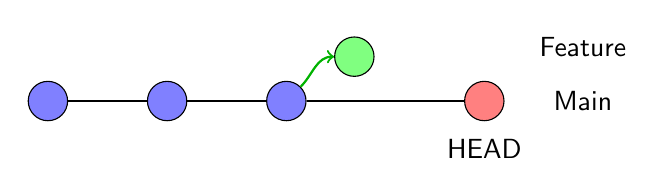
\begin{tikzpicture}[
        commit/.style={circle, draw, fill=blue!50, minimum size=0.5cm, inner sep=0pt},
        feature/.style={circle, draw, fill=green!50, minimum size=0.5cm, inner sep=0pt},
        head/.style={circle, draw, fill=red!50, minimum size=0.5cm, inner sep=0pt},
        line/.style={-, thick}
    ]
        % Main branch
        \node[commit] (c1) {};
        \node[commit, right=1cm of c1] (c2) {};
        \node[commit, right=1cm of c2] (c3) {};
        \node[head, right=2cm of c3] (c4) {}; % Gap for feature
        \node[right=0.5cm of c4] (end) {Main};
        
        \draw[line] (c1) -- (c2) -- (c3);
        \draw[line] (c3) -- (c4);
        
        % Feature branch
        \node[feature, above right=0.2cm and 0.5cm of c3] (f1) {};
        % \node[feature, right=1cm of f1] (f2) {};
        \node[above=0.2cm of end] (fend) {Feature};

        \draw[line, green!70!black, ->] (c3) to[out=45, in=180] (f1);
        % \draw[line, green!70!black] (f1) -- (f2);
        % \draw[line, green!70!black, ->] (f2) to[out=0, in=135] (c4);
        
        \node[below=0.1cm of c4] {HEAD};
        % \node[below=0.2cm of c4, font=\tiny] {Merge};
        
    \end{tikzpicture}
    \end{center}
\end{frame}

\begin{frame}[fragile]
    \frametitle{Merging Branches}
    Once the feature is complete and tested, merge it back into main.
    
    \vspace{0.3cm}
    \begin{minted}[fontsize=\small]{bash}
# while on the feature branch, commit your changes
git checkout feature
# ... make changes ...
git add .
git commit -m "Finished feature"
# Switch to main branch
git checkout main
# Merge feature branch into main
git merge feature
    \end{minted}
    \vspace{0.3cm}
    \begin{center}
    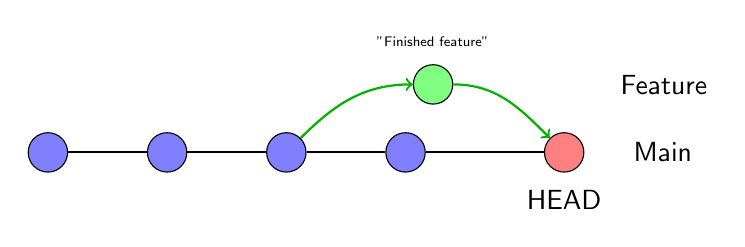
\begin{tikzpicture}[
        commit/.style={circle, draw, fill=blue!50, minimum size=0.5cm, inner sep=0pt},
        feature/.style={circle, draw, fill=green!50, minimum size=0.5cm, inner sep=0pt},
        head/.style={circle, draw, fill=red!50, minimum size=0.5cm, inner sep=0pt},
        line/.style={-, thick}
    ]
        % Main branch
        \node[commit] (c1) {};
        \node[commit, right=1cm of c1] (c2) {};
        \node[commit, right=1cm of c2] (c3) {};
        \node[commit, right=1cm of c3] (c5) {};
        \node[head, right=1.5cm of c5] (c4) {}; % Gap for feature
        \node[right=0.5cm of c4] (end) {Main};
        
        \draw[line] (c1) -- (c2) -- (c3) -- (c5);
        \draw[line] (c5) -- (c4);
        
        % Feature branch
        \node[feature, above right=0.5cm and 1.5cm of c3] (f1) {};
        % \node[feature, right=1cm of f1] (f2) {};
        \node[right=2cm of f1] (fend) {Feature};

        \draw[line, green!70!black, ->] (c3) to[out=45, in=180] (f1);
        % \draw[line, green!70!black] (f1) -- (f2);
        \draw[line, green!70!black, ->] (f1) to[out=0, in=135] (c4);
        
        \node[above=0.1cm of f1, font=\tiny] {"Finished feature"};
        \node[below=0.1cm of c4] {HEAD};
    \end{tikzpicture}
    \end{center}
\end{frame}

% \begin{frame}[fragile]
%     \frametitle{Creating a new branch}
%     \textbf{Create and switch to a new branch:}
%     \begin{minted}[fontsize=\small]{bash}
% git checkout -b new-branch-name
%     \end{minted}
%     \vspace{0.3cm}
%     \textbf{Switch back to an existing branch:}
%     \begin{minted}[fontsize=\small]{bash}
% git checkout branch-name
%     \end{minted}
% \end{frame}

\begin{frame}[fragile]
    \frametitle{Reverting with Reset (Advanced)}
    
    \begin{alertblock}{Warning}
        This can rewrite history. Use with caution.
    \end{alertblock}
    \textbf{Soft Reset:} Moves HEAD but keeps changes in Working Directory.
    \begin{minted}[fontsize=\small]{bash}
git reset --soft <commit-id>
    \end{minted}
    \vspace{0.3cm}
    \textbf{Hard Reset:} Moves HEAD and discards changes in Working Directory.
    \begin{minted}[fontsize=\small]{bash}
git reset --hard <commit-id>
    \end{minted}
\end{frame}

\begin{frame}
    \frametitle{Questions on Git so far?}
    \begin{center}
        Let's Try the interactive ``Visualizing Git'' demo in your browser to explore commits, branches and checkouts:
        
    \url{https://git-school.github.io/visualizing-git/}

    \vspace{0.5cm}

        \LARGE Any questions before we move on to GitHub?
    \end{center}
\end{frame}



%=============================================================
\section{GitHub \& Remotes}
%=============================================================

\begin{frame}
    \frametitle{Moving to the Cloud}
    
    \begin{center}
    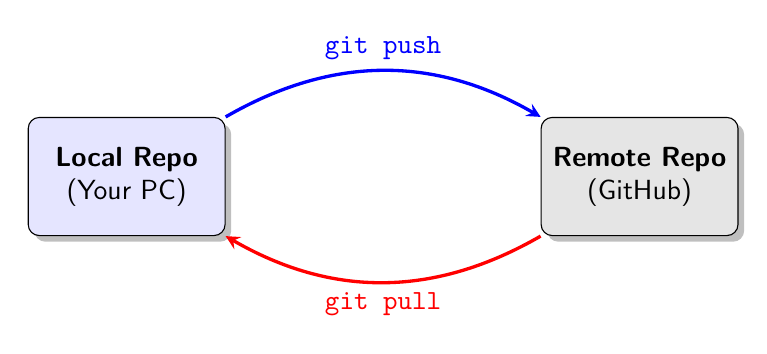
\begin{tikzpicture}[
        box/.style={draw, rectangle, rounded corners, minimum width=2.5cm, minimum height=1.5cm, align=center, fill=blue!10, drop shadow},
        arrow/.style={->, >=stealth, very thick}
    ]
        \node[box] (local) {\textbf{Local Repo}\\(Your PC)};
        \node[box, right=4cm of local, fill=gray!20] (remote) {\textbf{Remote Repo}\\(GitHub)};
        
        \draw[arrow, blue] (local.north east) to[out=30,in=150] node[midway, above, font=\ttfamily] {git push} (remote.north west);
        \draw[arrow, red] (remote.south west) to[out=210,in=330] node[midway, below, font=\ttfamily] {git pull} (local.south east);
    \end{tikzpicture}
    \end{center}
    
    \begin{itemize}
        \item \textbf{Origin:} The default nickname Git gives to your remote server.
        \item \textbf{Push:} Upload changes (Local $\rightarrow$ Remote).
        \item \textbf{Pull:} Download changes (Remote $\rightarrow$ Local).
    \end{itemize}
\end{frame}

\begin{frame}[fragile]
    \frametitle{Create Repo and Connecting to GitHub}
    
    \textbf{If you create a new existing local repo:}
    \begin{minted}[fontsize=\footnotesize]{bash}
    # 0. Initialize Git (if not done yet)
    git init
    # 1. Stage and commit your files
    git add .
    git commit -m "Initial commit"
    # 2. Link your local folder to GitHub (need to create
    # an empty repo on GitHub first)
    git remote add origin https://github.com/User/Repo.git
    # 3. Rename branch to 'main' (modern standard)
    git branch -M main
    # 4. Push your code!
    git push -u origin main
    \end{minted}
    
    \vspace{0.3cm}
    \textbf{If you are starting from an existing repo on GitHub:}

    \textbf{Clone} to download a repo from scratch (e.g., on a new PC):
    \begin{minted}[fontsize=\small]{bash}
    git clone <url>
    \end{minted}
\end{frame}

\begin{frame}[fragile]
    \frametitle{Pulling Changes}
    
    If others have pushed changes, you need to pull them first.
    
    \vspace{0.3cm}
    \textbf{Pull the latest changes:}
    \begin{minted}[fontsize=\small]{bash}
git pull origin main
    \end{minted}    
    \vspace{0.3cm}

    \begin{alertblock}{Good practice}
        Always pull before you push to avoid conflicts!
        
    \end{alertblock}
\end{frame}

\begin{frame}[fragile]
    \frametitle{Merging}
    If there are changes both locally and remotely, Git will try to merge them.

    \vspace{0.3cm}
    \textbf{Automatic Merge:} Git combines changes automatically.
    \begin{minted}[fontsize=\small]{bash}
git pull origin main
    \end{minted}    

    \vspace{0.3cm}
    \textbf{Manual Merge (Conflict):} If changes overlap, Git will mark conflicts in the files. You must resolve them manually.
    \begin{minted}[fontsize=\small]{bash}
# After resolving conflicts in files
git add conflicted-files # replace with actual file names
git commit -m "Resolved merge conflicts"
    \end{minted}
    
\end{frame}

\begin{frame}[fragile]
    \frametitle{Pull Requests}
    On GitHub, changes are often proposed via \textbf{Pull Requests (PRs)}.
    \begin{itemize}
        \item A way to review and discuss changes before merging them into the main branch.
        \item Typically used in collaborative projects.
        \item Enables code review, comments, and approval workflows.
    \end{itemize}
\end{frame}

\begin{frame}
    \frametitle{GitHub Features}
    \begin{itemize}
        \item \textbf{Issues:} Track bugs and feature requests.
        \item \textbf{Actions:} Automate workflows (e.g., testing, deployment).
        \item \textbf{Wiki:} Documentation for your project.
        \item \textbf{Projects:} Kanban boards for task management.
    \end{itemize}
\end{frame}

%=============================================================
% \section{Branching}
%=============================================================


\begin{frame}
    \frametitle{Your Turn Now!}
    
    \begin{enumerate}
        \item Open the Workshop1\_tasks.pdf file from blackboard
        \item Start working on the git/github exercises!
        \item Ask for help if you get stuck!
    \end{enumerate}
    
\end{frame}

\end{document}